\subsection{Принужденное изменение порядка ключей}
\label{sec:optimization:key_ordering}

Для понимания текущей проблемы стоит рассмотреть пример:

\begin{lstlisting}[language=Prolog]
fcst_in_range[sku, store, week] = f <-
  fcst[sku, store, week]=f,
  future_week(week).
\end{lstlisting}

Поскольку одной из идей платформы является выполнение операции \join сразу по всем ключам, то оптимизатор запроса должен выбрать необходимый порядок ключей, чтобы выполнить фильтрацию, в случаях выполнения или поддержания правила. В качестве ключей выступают все переменные в выражениях в теле правила. Алгоритм является эвристическим и направлен на то, чтобы как можно раньше отфильтровать объекты. Этот подход легко объясняется - чем раньше происходит фильтрация, тем меньше данных нужно будет обработать для выполнения \join. Возможные следующие варианты порядка ключей:

\begin{itemize}
  \item \lstinline{[sku, store, week]};
  \item \lstinline{[week, sku, store]};
  \item могут быть другие варианты, но они, очевидно, хуже.
\end{itemize}

На рисунке \ref{fig:optimization:key_ordering:key_ordering_choice} представлен пример размещения страниц с данными для предиката \lstinline{fcst_in_range}. Далее, на рисунке \ref{fig:optimization:key_ordering:key_ordering_choice_join}, уже показана попытка сделать \join для ключа \lstinline{week}. Как видно, чтобы это осуществить, необходимо проитерироваться \emph{по всем} страницам предиката, поскольку ключ \lstinline{week} идет в нем последним. Поэтому выбор порядка ключей \lstinline{[week, sku, store]} неудачен и оптимизатор сделает предпочтение \lstinline{[sku, store, week]}.

\begin{figure}
	\centering
	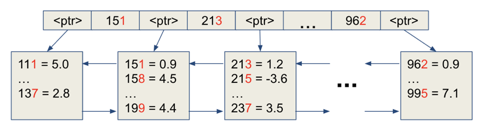
\includegraphics[scale=0.9]{key_ordering_choice.png}
	\caption{Пример представления страниц в памяти для предиката \lstinline{fcst_in_range}}
	\label{fig:optimization:key_ordering:key_ordering_choice}
\end{figure}

\begin{figure}
	\centering
	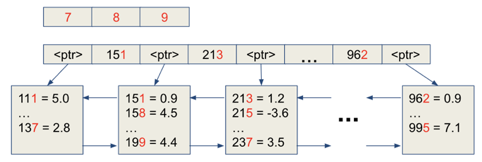
\includegraphics[scale=0.9]{key_ordering_choice_join.png}
	\caption{Выполнения операции \join по ключу \lstinline{week}}
	\label{fig:optimization:key_ordering:key_ordering_choice_join}
\end{figure}

Рассмотрим следующую проблему. Пусть в некотором предикате (в силу решения проблемы случайных вставок) порядок ключей определен как \lstinline{[week, sku, store]}, а в другом - \lstinline{[sku, store, week]}, и их необходимо слить. Для этого необходимо воспользоваться индексом. В данном случае понадобится инвертированный индекс \cite{inverted_index}, который позволит одному из предикатов перейти к другому порядку ключей. Такой индекс создается \emph{автоматически} исполняющей средой, если на то есть необходимость. Из плюсов:

\begin{itemize}
  \item помогает быстро отвечать на запросы разного порядка ключей.
\end{itemize}

Минусы:

\begin{itemize}
  \item его необходимо поддерживать (дублировать data modification операции с исходного предиката);
  \item он занимает столько же памяти, сколько и исходный предикат.
\end{itemize}

Рассмотрим пример. При выполнении кода выше среда может добавить инвертированный индекс, и правило перезапишется следующим образом:

\begin{lstlisting}[language=Prolog]
fcst_in_range[sku, store, week] = f <-
   fcst$2_0_1_3[week, sku, store] = f,
   future_week(week).
\end{lstlisting}

Здесь инвертированный индекс \lstinline{fcst$2_0_1_3} (такие индексы всегда имеют такие названия с порядком ключей, чтобы давать информацию о себе, встречая его впервые и не лезя в детали) выглядит так:

\begin{lstlisting}[language=Prolog]
fcst$2_0_1_3[week, sku, store] = f <-
  fcst[sku, store, week] = f.
\end{lstlisting}

Создание и использование индексов скрыто от разработчика - это все решает среда выполнения. Чтобы отыскать детали использования индексов, стоит смотреть в специальные логи.

Как и в других ситуациях, решение с индексами не дает исключительных выгод. Есть и серьезные недостатки:

\begin{enumerate}
  \item Поскольку они создаются автоматически (разработчик не может это контролировать), при некоторых долгих запросах пользователь может ждать дольше, чем обычно, из-за создания индекса.
  \item Как упоминалось, индексы занимают примерно столько же памяти, сколько и исходные предикаты.
  \item В некоторых случаях, когда индекс создается в readonly транзакциях, он не будет поддерживаться в дальнейшем при изменениях исходного предиката. В таких ситуациях индекс удаляется при следующей операции изменения, что занимает временные ресурсы. Поэтому если изменять большой по размеру предикат, а затем делать на нем запросы, требующие индекса, такой индекс будет создаваться и удаляться каждый раз.
\end{enumerate}

Управление индексами в процессе выполнения скрыто для разработчика. Единственное, что можно сделать, это создание индексов заранее. Такое решение оправдано, когда заранее можно быть увереным, что среда будет часто пересоздавать индекс, либо просто выгодно создать его именно во время разворачивания всей системы, а не в процессе выполнения. Для этого индексы описываются в специальном файле \lstinline{scripts/indexes.txt}. Среди проблем такого подхода:

\begin{itemize}
  \item использование индекса замедляет обновления;
  \item скорее всего с ними порядок ключей будет выбран неподходяще.
\end{itemize}

Исходя из таких рассуждений можно вынести следующие рекомендации:

\begin{enumerate}
  \item стоит заранее создавать индексы на предикаты, которые не обновляются с \ui;
  \item индексирование большого предиката, которые обновляется с \ui - очень плохая идея;
  \item чтобы избавить от необходимости создавать индексы, стоит прибегнуть к переупорядочиванию ключей в теле предиката, но такое решение требует тщательного тестирования.
\end{enumerate}

Чтобы помочь системе правильно использовать индексы, можно подсказывать ей и изменять порядок используемых ключей. Рассмотрим на примере:

\begin{lstlisting}[language=Prolog]
filtered_fcst[sku, store, week]=f <-
  forecast[sku, store, week]=f,
  filter(sku, store),
  fcst_horizon(week).
\end{lstlisting}

И наложим ограничения (для примера):

\begin{itemize}
  \item \lstinline{fcst_horizon} содержит 52 записи (текущая неделя и на год вперед);
  \item \lstinline{filter} содержит 100.000 записей, но довольно разрежен по параметру \lstinline{sku};
  \item оптимизатор выберет порядок ключей как \lstinline{(week, sku, store)}. Заранее скажем, что это плохой выбор порядка ключей, так как кроме построения индекса, \lstinline{filter} по факту не сделает большой работы по самой фильтрации.
\end{itemize}

Итак, исходя из некоторых соображений (возможно, мы знаем, как предикаты могут фильтровать друг друга, или мы хотим не давать системе создавать большой индекс), мы создаем прагму:

\begin{lstlisting}[language=Prolog]
pragma_force_key_ordering(sk, st, wk) ->
  sku(sk), loc(st), week(wk).
\end{lstlisting}

Прагма явно задает порядок ключей, который оптимизатор должен выбрать. Теперь мы можем использовать данную прагму в нашем правиле:

\begin{lstlisting}[language=Prolog]
fcst_in_range[sku, store, week] = f <-
  pragma_force_key_ordering(sku, store, week),
  fcst[sku, store, week]=f,
  filter(sku, store),
  future_week(week).
\end{lstlisting}

В этом случае, оптимизатор однозначно определит порядок ключей как \lstinline{[sku, store, week]}. Но, как ни странно, широкое использование прагм может привести к ухудшению ситуации:

\begin{itemize}
  \item все-таки это ограничение на оптимизатор, и в большинстве случаев оптимизатор использует более правильный подход;
  \item следует избегать при существовании другого решения;
  \item обычно стоит переформулировать правило и использовать новый материализованный предикат вместо изменения порядка ключей.
\end{itemize}
